% To je predloga za poročila o domačih nalogah pri predmetih, katerih
% nosilec je Blaž Zupan. Seveda lahko tudi dodaš kakšen nov, zanimiv
% in uporaben element, ki ga v tej predlogi (še) ni. Več o LaTeX-u izveš na
% spletu, na primer na http://tobi.oetiker.ch/lshort/lshort.pdf.
%
% To predlogo lahko spremeniš v PDF dokument s pomočjo programa
% pdflatex, ki je del standardne instalacije LaTeX programov.

\documentclass[a4paper,11pt]{article}
\usepackage{a4wide}
\usepackage{fullpage}
\usepackage[utf8x]{inputenc}
\usepackage[slovene]{babel}
\selectlanguage{slovene}
\usepackage[toc,page]{appendix}
\usepackage[pdftex]{graphicx} % za slike
\usepackage{setspace}
\usepackage{color}
\definecolor{light-gray}{gray}{0.95}
\usepackage{listings} % za vključevanje kode
\usepackage{hyperref}
\renewcommand{\baselinestretch}{1.2} % za boljšo berljivost večji razmak
\renewcommand{\appendixpagename}{Priloge}

% Default fixed font does not support bold face
\DeclareFixedFont{\ttb}{T1}{txtt}{bx}{n}{10} % for bold
\DeclareFixedFont{\ttm}{T1}{txtt}{m}{n}{10}  % for normal

\definecolor{deepblue}{rgb}{0,0,0.5}
\definecolor{deepred}{rgb}{0.6,0,0}
\definecolor{deepgreen}{rgb}{0,0.5,0}

\lstset{ % nastavitve za izpis kode, sem lahko tudi kaj dodaš/spremeniš
language=Python,
basicstyle=\ttm,
otherkeywords={self},             % Add keywords here
keywordstyle=\ttb\color{deepblue},
emph={MyClass,__init__},          % Custom highlighting
emphstyle=\ttb\color{deepred},    % Custom highlighting style
stringstyle=\color{deepgreen},
breaklines=true,
postbreak=\mbox{\textcolor{red}{$\hookrightarrow$}\space},
}

\title{%
  Vaja 4 - Potapljanje ladjic\\
  \large Postavitev in upravljanje računalniških oblakov}
\author{David Rubin \\ (david.rubin@student.um.si)}
\date{\today}

\begin{document}

\maketitle

\section{Opis naloge}

Implementirati je bilo potrebno MPI program, ki izvaja večigralsko potaplanje ladjic. Slednje je izvedeno tako, da je neko vozlišče gospodar (v mojem primeru \textit{trusty0}), ki hrani stanje igre in sprašuje igralce po njihovih potezah. To vozlišče skrbi tudi za spletni strežnik, ki omogoča vpogled v stanje med igranjem igre.

\section{Opis rešitve}

Rešitev sem implementiral kot Vagrant konfiguracijo gruče, skripto za kopiranje programa na vse instance in Python MPI program opisanega potaplanja ladjic. V Vagrant datoteki se namesti vse potrebno (\textit{mpi4py, nginx} ipd.) v 10 instanc okolja Ubuntu 14.04 Trusty Tahr. Poskrbi tudi za povezljivost med instancami, kot tudi za fiksno določene IP naslove.

Skripta za kopiranje programa iz datoteke prebere IP naslove vseh 10 strežnikov in podan parameter (ime programa) prekopira na vsako izmed njih.

Program napisan v Pythonu je viden v kodnem bloku~\ref{battleships}. Skratka, vzpostavi se igralno polje in kopija tega, ki drži pozicije ladjic, ki so fiksno določene. Potem glavno vozlišče pošlje polje vsem ostalim, ti pa odgovorijo z naključno izbranimi koordinatami, ki pa se preverijo, da so še neigrana polja. Ko se potopi zadnja ladjica, glavno vozlišče namesto polja vsem igralcem pošlje vrednost -1, ki zaključi igro. Na gospodarju se izpišejo rezultati igralcev in program se zaključi.

\lstinputlisting[language=python,label=battleships,caption=Program za večigralsko potaplanje ladjic,firstline=14]{battleships.py}

Med kodo lahko opazimo tudi HTML, na gospodarju imamo namreč nameščen spletni strežnik nginx, kateremu pa smo spremenili konfiguracijo, da streže datoteko ~/www/index.html. Vsebino te datoteke spreminjamo z zgoraj navedenim programom. Na sliki~\ref{slika1} vidimo spletni vmesnik programa med izvajanjem igre, na sliki~\ref{slika2} je spletni vmesnik po končani igri, na sliki~\ref{slika3} pa je viden še ukaz, ki je pognal igro.

\begin{figure}
\begin{center}
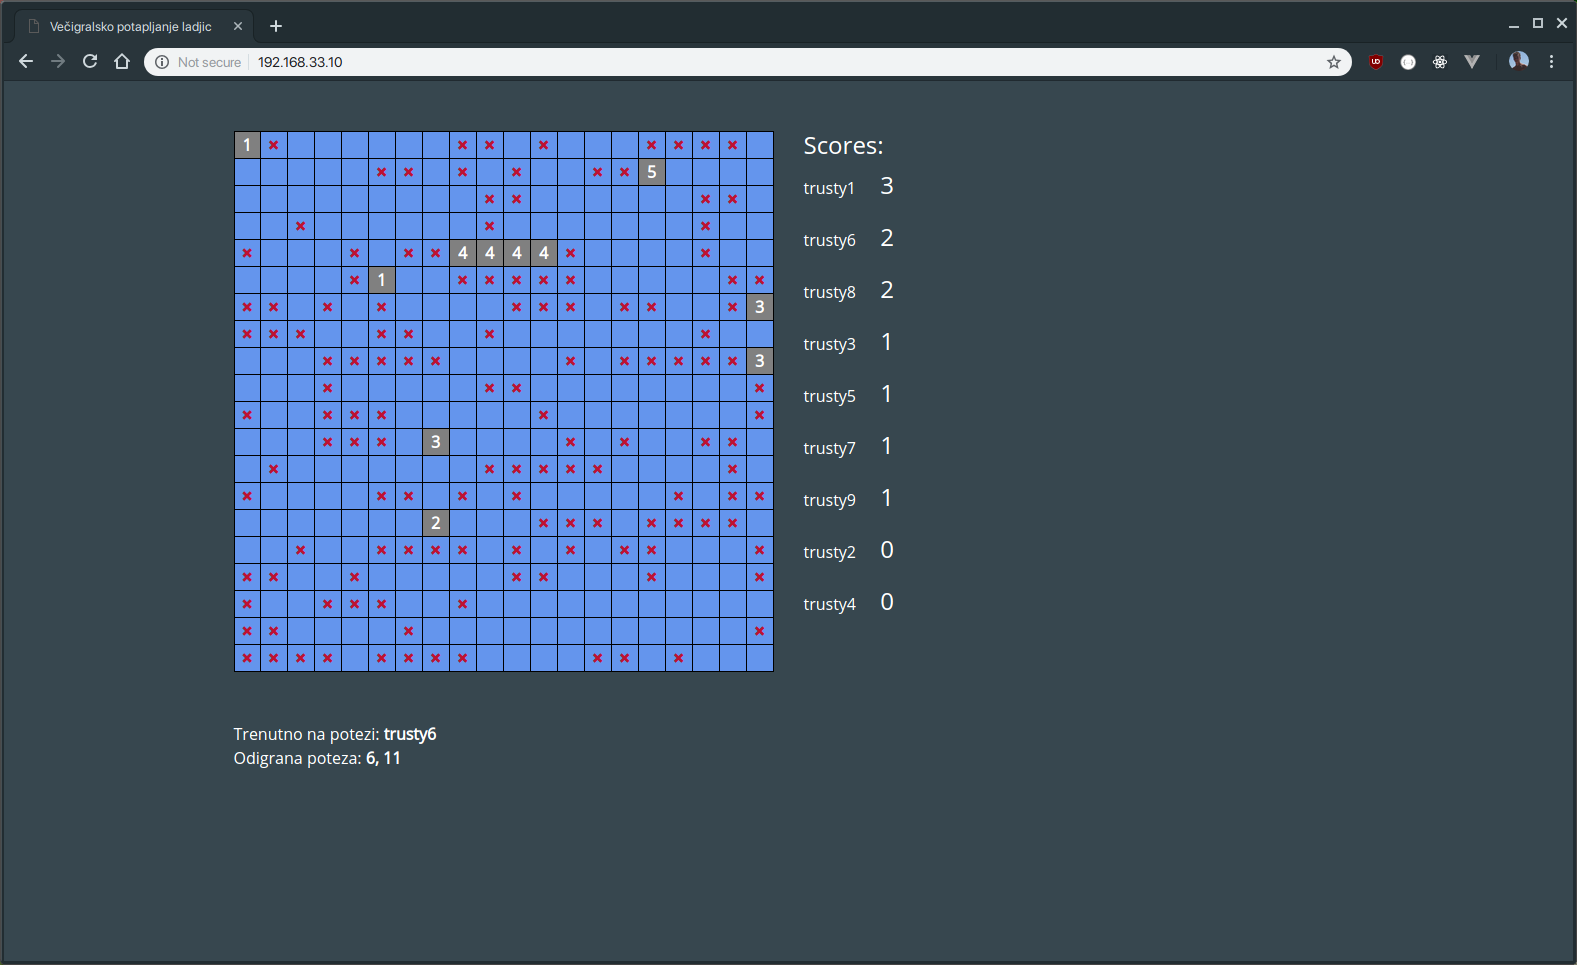
\includegraphics[scale=0.4]{./midgame.png}
\caption{Spletni vmesnik med igranjem igre}
\label{slika1}
\end{center}
\end{figure}

\begin{figure}
\begin{center}
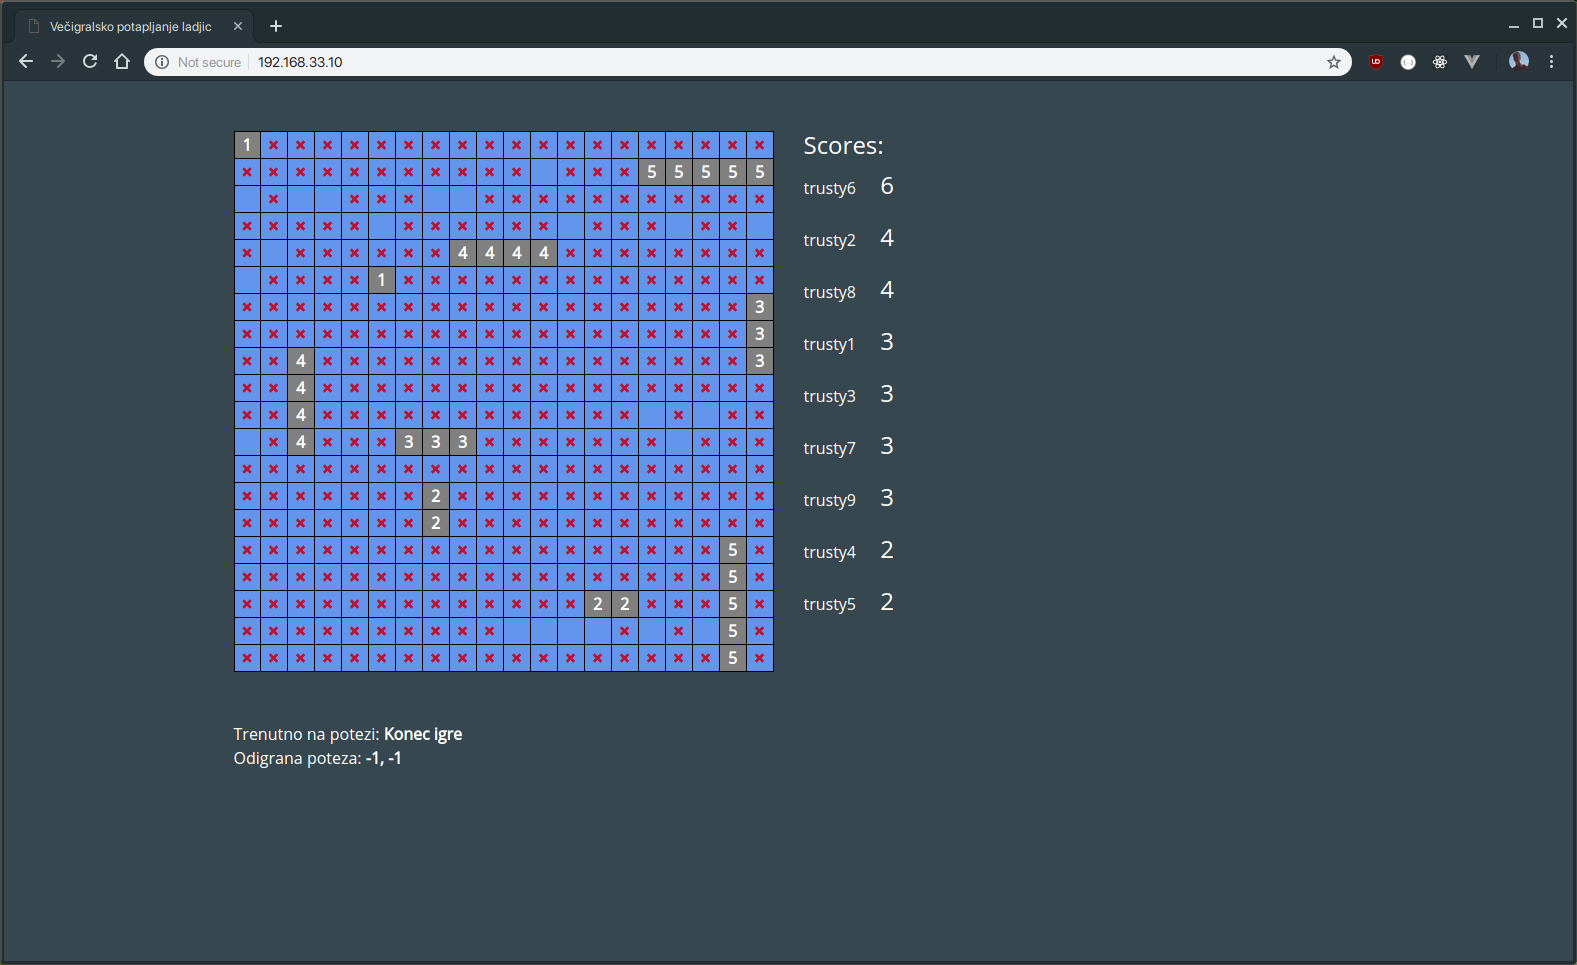
\includegraphics[scale=0.4]{./endgame.png}
\caption{Spletni vmesnik po končani igri}
\label{slika2}
\end{center}
\end{figure}

\begin{figure}
\begin{center}
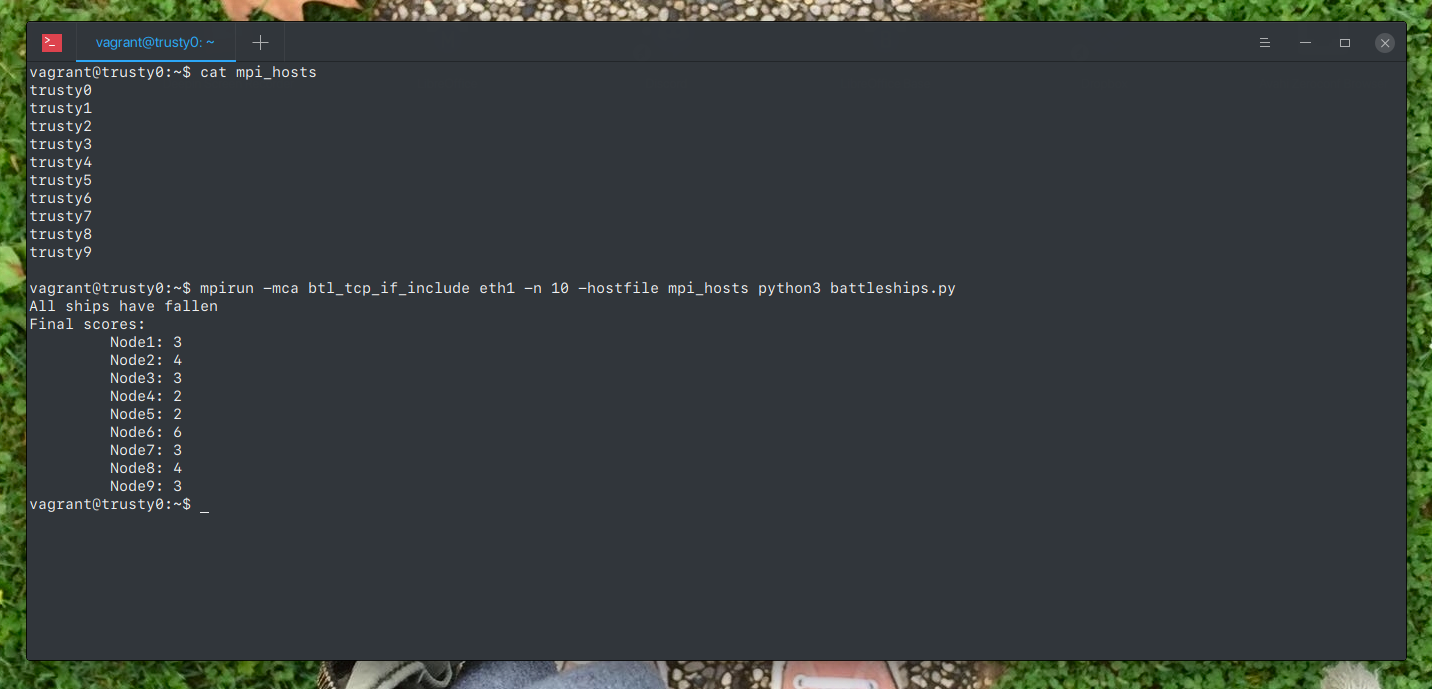
\includegraphics[scale=0.45]{./commands.png}
\caption{Zaključen ukaz, ki je pognal zgoraj prikazano igro}
\label{slika3}
\end{center}
\end{figure}

\section{Izjava o izdelavi domače naloge}
Domačo nalogo in pripadajoče programe sem izdelal sam.

\end{document}
